\documentclass{beamer}

\usetheme{Singapore}

\usepackage{float}
\usepackage{multimedia}
\usepackage{color}
\usepackage{polski}
\usepackage[utf8]{inputenc}

\title{Wyrażenia regularne - regex}
\author{Ewa Namysł}
\institute{Uniwersytet Śląski}
\date{10 marca 2022}

\begin{document}

%STRONA TYTUŁOWA
\frame{
	\titlepage
}

%SPIS TREŚCI
\frame{
	\tableofcontents
	\frametitle{Spis treści}
}

%WSTĘP
\section{Czym są wyrażenia regularne?}
\frame{
	\frametitle{Czym są wyrażenia regularne?}
	\centering

	\textbf{Wyrażenia regularne}, w skrócie regex,\\
	to wzorce opisujące łańcuchy symboli.\\
	\vspace{1em}
	Upraszczając, jest to zbiór zasad opisujących\\
	jakiś tekst, zestaw znaków i cyfr etc.
}

\frame{
	\frametitle{Historia}
	\centering

	 W 1951 roku matematyk Stephen Cole Kleene stworzył podwaliny teorii opisującej języki regularne używając notacji matematycznej.\\
	\vspace{1em}
	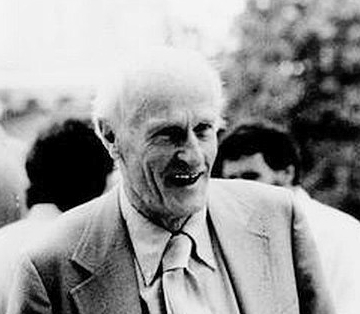
\includegraphics[scale=0.45]{kleene.jpg}
}

\frame{
	\centering

	Regex zyskał na popularności pod koniec lat sześćdziesiątych wraz z rozwojem Unixa.\\
	\vspace{1em}
	Ken Thompson, współtwórca Unixa, jako jeden z pierwszych wykorzystał notację Kleene'a w edytorze tekstu \textit{QED}.\\
	\vspace{0.5em}
	Thompson stworzył również na własny użytek narzędzie wyszukujące pliki według wzorców regexa.\\
	Obecnie znamy to narzędzie pod nazwą \textit{grep}.
	\vspace{2em}
	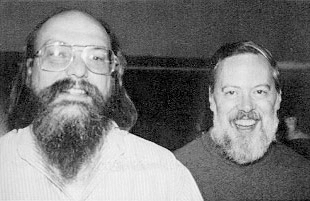
\includegraphics[scale=0.45]{thompson_ritchie.jpg}
}

\frame{
	\frametitle{Co zyskujemy?}
	\centering
	
	Dzięki wyrażeniom regularnym jesteśmy w stanie odnaleźć w tekście wszystkie wystąpienia danego wzorca.\\
	\vspace{1em}
	Jeśli poszukujemy konkretnego słowa, odnajdziemy je jako osobny string, ale również jeśli występuje jako składowa część wyrazu.
}

\frame{
	\frametitle{Przykład}
	\centering

	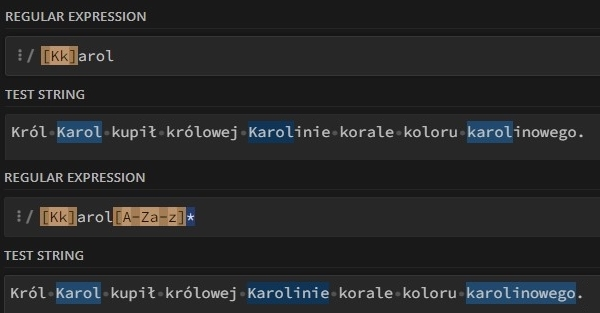
\includegraphics[scale=0.5]{przyklad1.jpg}
}


\frame{
	\frametitle{Popularne zastosowania}

	\begin{itemize}
		\item Walidacja danych - sprawdzanie adresów mailowych, kodów pocztowych, siły haseł etc.
		\item Webscraping - zautomatyzowane pozyskiwanie danych ze stron internetowych.
		\item Modyfikacja i podmienianie łańcuchów znaków, obróbka danych.
		\item Edytory tekstu, kompilatory.
	\end{itemize}
}

\frame{
	\centering

	Wiele programów i komend Linuxa wykorzystuje regexy, m.in.\\
	\textit{grep}, \textit{sed}, \textit{find}.\\
	\vspace{1em}
	Większość współczesnych języków programowania ma własne biblioteki obsługujące regexy, np. \textit{re} w Pythonie.
}

%SKŁADNIA
\section{Podstawy składnii i przykłady}

\frame{
	\frametitle{Podstawy składni - kwadratowe nawiasy}
	\centering
	
	\begin{itemize}
		\item $[ ] \rightarrow$ wybiera jeden ze znaków wewnątrz nawiasów, np.
	\end{itemize}
		[abc] wyszuka litery a, b lub c.
	\begin{itemize}
		\item $[A-Za-z] \rightarrow$ dowolna wielka lub mała litera.
		\item $[0-9] \rightarrow$ jedna cyfra od 0 do 9
		\item $[\string^] \rightarrow$ zaprzeczenie znaków wewnątrz nawiasu, np.
	\end{itemize}
	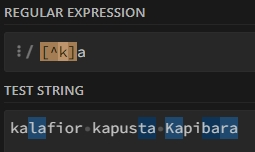
\includegraphics[scale=0.6]{kapibara.jpg}
}

\frame{
	\frametitle{Krótszy zapis}

	\begin{itemize}
		\item \textbackslash{d} $\rightarrow$ jeden znak, który jest cyfrą
		\item \textbackslash{D} $\rightarrow$ jeden znak, który NIE jest cyfrą
		\item \textbackslash{w} $\rightarrow$ jeden znak, który jest literą
		\item \textbackslash{W} $\rightarrow$ jeden znak, który NIE jest literą
		\item \textbackslash{s} $\rightarrow$ jeden znak, który jest białym znakiem
		\item \textbackslash{S} $\rightarrow$ jeden znak, który NIE jest białym znakiem
	\end{itemize}
}

\frame{
	\frametitle{Podstawy składni - znaki specjalne i kwantyfikatory}
	\centering

	\begin{itemize}
		\item $\cdot \rightarrow$ jeden dowolny znak (oprócz znaków nowej linii), np.
	\end{itemize}
	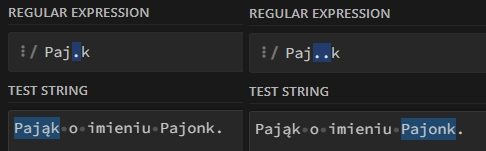
\includegraphics[scale=0.5]{pajonk.jpg}
}

\frame{
	\centering

	\begin{itemize}
		\item * $\rightarrow$ zero lub więcej powtórzeń znaku, np.
	\end{itemize}
	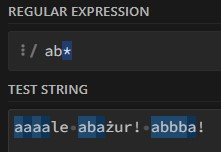
\includegraphics[scale=0.5]{ale_abazur_gwiazdka.jpg}
	\begin{itemize}
		\item + $\rightarrow$ jedno lub więcej powtórzeń znaku, np.
	\end{itemize}
	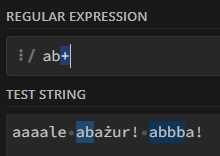
\includegraphics[scale=0.4]{ale_abazur_plus.jpg}
	\begin{itemize}
		\item ? $\rightarrow$ zero lub jedno powtórzenie znaku, np.
	\end{itemize}
	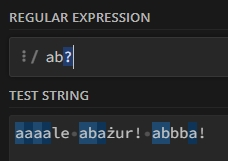
\includegraphics[scale=0.4]{ale_abazur_pytajnik.jpg}
}

\frame{
	\centering

	\begin{itemize}
		\item $\{\} \rightarrow$ określona liczba powtórzeń znaku, np.
	\end{itemize}
	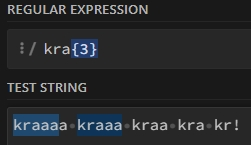
\includegraphics[scale=0.4]{kra1.jpg}
	\begin{itemize}
		\item $\{min, max\} \rightarrow$ zakres powtórzeń znaku
	\end{itemize}
	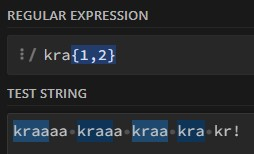
\includegraphics[scale=0.55]{kra2.jpg}
}

\frame{
	\frametitle{Kotwice}
	\centering

	\begin{itemize}
		\item $\string^ \rightarrow$ szuka na początku tekstu podanego ciągu znaków, np.
	\end{itemize}
	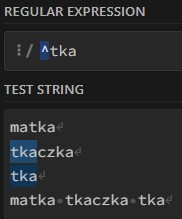
\includegraphics[scale=0.55]{daszek.jpg}
	\begin{itemize}
		\item $\$ \rightarrow$ szuka na końcu tekstu podanego ciągu znaków, np.
	\end{itemize}
	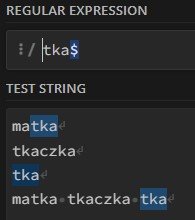
\includegraphics[scale=0.55]{dolar.jpg}
}

\frame{
	\centering

	\begin{itemize}
		\item $\string^$ oraz \$ można też łączyć. Regex wyszuka wówczas tekst, który od początku do końca pasuje do wzorca:
	\end{itemize}
	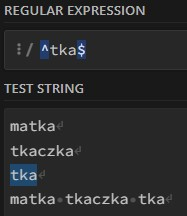
\includegraphics[scale=0.55]{daszekdolar.jpg}
}

\frame{
	\centering

	\begin{itemize}
		\item  \textbackslash{b} $\rightarrow$ znajduje granicę słów.
	\end{itemize}
	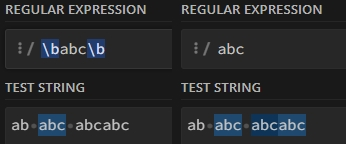
\includegraphics[scale=0.6]{rushb.jpg}
}

\frame{
	\frametitle{Alternatywa}
	\centering

	\begin{itemize}
		\item $\mid \rightarrow$ umożliwia użycie alternatywy:
	\end{itemize}
	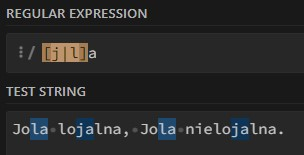
\includegraphics[scale=0.7]{jola.jpg}
}

%PRZYKŁADY W PRAKTYCE
\section{Proste przykłady w praktyce}
\frame{
	\frametitle{Python}
	\centering
	
	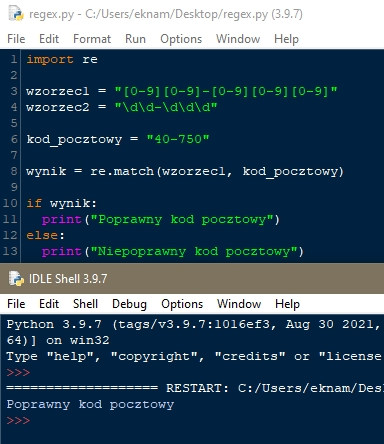
\includegraphics[scale=0.5]{python.jpg}
}

\frame{
	\frametitle{Linux}
	\centering
	
	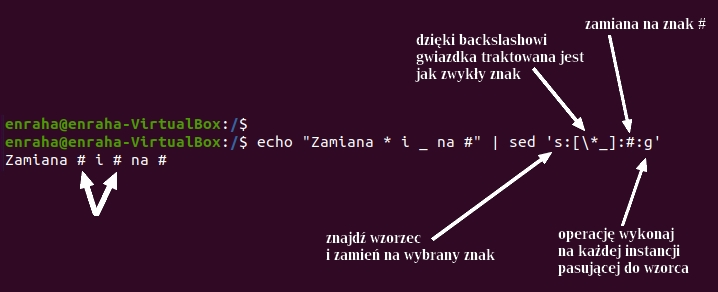
\includegraphics[scale=0.45]{linux.jpg}
}

%PODSUMOWANIE
\section{Podsumowanie}
\frame{
	\frametitle{Wady}
	\centering

	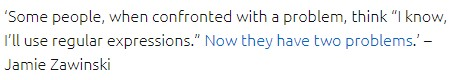
\includegraphics[scale=0.9]{ubuntu.jpg}
	\vspace{1em}
	\begin{itemize}
		\item Bardzo złożona składnia, podatność na pomyłki i fałszywie pozytywne wyniki.
		\item Ekstremalnie trudny do modyfikacji dla osoby, która go nie pisała.
		\item Zasobożerny.
	\end{itemize}
}

\frame{
	\frametitle{Zalety}
	\centering

	\begin{itemize}
		\item Często krótsze, mniej rozbudowane rozwiązanie dla bieżących problemów (choć niekoniecznie szybciej na nie wpadniemy).
		\item Współpraca z komendami Linuxa.
		\item W niektórych sytuacjach (np. loginy userów, wprowadzanie tekstu przez usera) może okazać się niezastąpiony przez swoją elastyczność.
	\end{itemize}
}

\frame{
	\frametitle{Bibliografia:}

	J. Goyvaerts, \emph{Regular Expressions}, https://www.regular-expressions.info/ (dostep kwiecień 2022).\\
	\vspace{1em}
	R. Winslow, \emph{Regex basics}, https://ubuntu.com/blog/regex-basics/ (dostęp kwiecień 2022).\\
	\vspace{1em}
	M. Mamczur, \emph{Wyrażenia regularne – czym są i jak pisać własne regex’y?}, https://miroslawmamczur.pl/wyrazenia-regularne-czym-sa-i-jak-pisac-wlasne-regexy/ (dostęp kwiecień 2022).\\
	\vspace{1em}
	\emph{Regular Expressions 101}, https://regex101.com/, (dostęp kwiecień 2022).
}

\end{document}